\chapter{Аналитический раздел}

В данном разделе проводится исследование подходов к синтезу реалистичных изображений, осуществляется описание сцены, трехмерных объектов в сцене, проводится сравнительный анализ различных алгоритмов и обзор существующих решений.

\section{Описание сцены}

В компьютерной графике сцена является неотъемлемым компонентом, содержащим в себе всю информацию, необходимую для синтеза изображения. Поэтому определение ее структуры является одним из важнейших и первостепенных шагов в создании программы.

В реализовываемом программном продукте сцена будет представлена структурой, содержащей в себе коллекцию из объектов и коллекцию из источников освещения. Размеры этих коллекций будут ограничены лишь объемом оперативной памяти.

\section{Описание моделей трехмерных объектов в сцене}

Существует множество способов представления трехмерных объектов в сцене. Различным алгоритмам отрисовки требуется разная информация о самом объекте.

\subsection{Функциональное моделирование}

Одним из простейших способов задания трехмерных объектов можно назвать функциональное моделирование. Возможно несколько вариантов.

\begin{enumerate}
    \item Поверхность такого объекта задается системой уравнений:
	\begin{equation}
		\left\{
		\begin{array}{l}
			x = x(u, v) \\
			y = y(u, v) \\
			z = z(u, v) \\
		\end{array}
		\right.,
	\end{equation}

    в этом случае каждая точка на поверхности объекта из плоской системы координат $(u, v)$ преобразуется в мировое пространство $(x, y, z)$.

    \item Внутренний объем такого объекта выражается неравенством:
    \begin{equation}
        f(x, y, z) > 0.
    \end{equation}
    
    Данное неравенство справедливо для всех точек внутри объекта.
\end{enumerate}

Особенности данного представления:

\begin{itemize}
    \item функциональное моделирование позволяет получить максимальный уровень детализации при отрисовке, наилучшую сглаженность формы объекта;
    \item достаточно сложная форма может иметь довольно простое параметрическое представление, из чего следует меньший расход памяти при хранении представления объекта;
    \item трансформации над объектом производятся очень просто. Достаточно применить преобразования к описывающим объект уравнениям или неравенствам;
    \item наложение текстур в случае с внутренне-определёнными объектами является затруднительным;
    \item процесс отыскания параметрического представления невыпуклых многогранников может быть затруднительным.
\end{itemize}

\subsection{Полигональная сетка}

Полигональная сетка состоит из набора отдельных полигонов, которые в свою очередь являются многоугольниками, ребра которых соединяют вершины сетки. \cite{polygon-net}. Структура полигональной модели представлена ниже, на рисунке \ref{pic:polygon-net}

\begin{figure}[h]
	\centering
	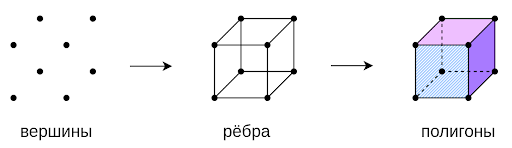
\includegraphics[width=0.8\linewidth]{inc/img/polygon-model.png}
	\caption{Структура полигональной модели.}
	\label{pic:polygon-net}
\end{figure}

Полигональная сетка является аппроксимацией поверхности представляемого объекта. От её плотности, т.е. от количества полигонов на единицу объема, зависит качество изображения объекта.

Особенности данного представления:

\begin{itemize}
	\item просто создать топологию поверхности;
	\item преобразования над объектом сводятся к преобразованию полигональной сетки, что в свою очередь раскладывается на независимые преобразования над отдельными полигонами;
	\item наложение текстур на поверхность является несложной процедурой;
	\item повышение плотности сетки приводит к увеличению объема затрачиваемой памяти для ее хранения.
\end{itemize}

\clearpage

\subsection{Воксельная сетка}

Воксел -- это элемент объема. Воксельная модель разбивает весь объем трехмерного изображения на ячейки -- вокселы, создавая трехмерный растр \cite{voxel}.
